\section{Review on Graph Theory  \cite{agnarsson2006graph}}
\subsection{Preliminaries}
\begin{itemize}
\item \textbf{set} - a group of objects
\item \textbf{element} - an object inside a set
\item \textbf{empty set} - null set;contains no element; denoted by $\varnothing$ or $\{\}$
\item If n element $a$ is in set $S$, then $a \in S $.
\item If a set $t$ contains some or all the elements of a set S, then $t \subseteq S$.
\item If set $S$ contains all the elements of $T$ and vice-versa, then $t=S$.
\item Let $A$ and $B$ be sets,
\begin{itemize}
	\item $A \cup B$ or the \textit{union of A and B} is the set containing all the element/s of both set $A$ and set $B$.
	\item $A \cap B$ or the \textit{intersection of A and B} is the set containing the element/s that are present in both set $A$ and set $B$.
	\item set $A$ and set $B$ are disjoint sets if they have no same elements. Disjoint sets can be written as $A \cap B=\varnothing$.
	\item $A \setminus B$ or the \textit{set difference of A and B} is the set containing all the elements of $A$ that are not in $B$.
	\item $A \Delta B$ or the \textit{symmetric difference of A and B} is equal to $(A \setminus B) \cup (B \setminus A)$. 
\end{itemize}
 \item \textbf{finite set} - a countable set; set that contains countable number elements
 \item  \textbf{cardinality of set $S$ or $|S|$} - the number of elements of set $S$
 \item \textbf{power set of $S$ or $P(S)$} - the set that all the possible subsets of S including the empty set
 \item Let $k \in \mathbb{N}$ and $a_1,a_2,...,a_k$ are any k number of objects; \textit{ordered k-tuple or k-tuple} can be written as $(a_1,a_2,...,a_k)$.
 \item Some sets of numbers:
 \begin{itemize}
 	\item set of natural numbers or $\mathbb{N} = \{1,2,3,...\}$
 	\item integer set or $\mathbb{Z} = \{...,-2,-1,0,1,2,...\}$
 	\item set of rational numbers or $\mathbb{Q} = \{a/b:a,b \in \mathbb{Z},b\neq 0 \}$
 	\item set of real numbers or $\mathbb{R}$
 \end{itemize}
\end{itemize}

\subsection{Graphs}
\begin{itemize}
 \item \textbf{graph or general graph} - ordered triple $G=(V,E,\phi)$ where, $V\neq\emptyset$, $V \cap E = \emptyset$ and $\phi:E \rightarrow P(V)$ such that the cardinality of $\phi$ is either 1 or 2 for every $e \in E$.
 \item Let G be a graph with $G = (V,E,\phi)$,
	\begin{itemize}
		\item The vertex set or $V$ is the set of vertices of G
		\item The edge set or $E$ is the set of edges
		\item $\phi(e)$ contains the endvertex/endvertices of each $e$ which are the elements of the vertex set. 
	\end{itemize}	 
\begin{figure}[h]
\centering
\begin{tikzpicture}[-,>=stealth',shorten >=1pt,auto,node distance=3cm,
                    thick,main node/.style={circle,draw,font=\sffamily\Large\bfseries}]

  \node[main node] (1) {$v_1$};
  \node[main node] (2) [below left of=1] {$v_2$};
  \node[main node] (3) [below of=1] {$v_3$};
  \node[main node] (4) [below right of=1] {$v_4$};
  \node[main node] (5) [below of=3] {$v_5$};
  \node[main node] (6) [right of=4] {$v_6$};
  
  \path[every node/.style={font=\sffamily\large}]
    (1) edge node [right] {$e_3$} (4)
    	edge node [left] {$e_1$} (2)
    	edge node {$e_2$} (3)
    (2) edge [loop left] node {$e_6$} (2)
    (3) edge node [right] {$e_4$} (5)
        edge node [right] {$e_7$} (4)
    (4) edge node {$e_5$} (5)
	(5) 
    ;
\end{tikzpicture}
\caption{Graph G with 6 vertices and seven edges.}
\label{graph1}
\end{figure}
In figure \ref{graph1}, 
\begin{equation}
\begin{array}{l}
G=(V,E,\phi) \\
V=\{v_1,v_2,v_3,v_4,v_5,v_6\} \\
E=\{e_1,e_2,e_3,e_4,e_5,e_6,e_7\} \\
\phi(e_1)=\{v_1,v_2\} \\
\phi(e_2)=\{v_1,v_3\} \\
\phi(e_3)=\{v_1,v_4\} \\
\phi(e_4)=\{v_3,v_5\} \\
\phi(e_5)=\{v_4,v_5\} \\
\phi(e_6)=\{v_2,v_2\} \\
\phi(e_7)=\{v_3,v_4\}
\end{array}
\end{equation}
Let the graph $G=(V,E,\phi)$,
	\begin{itemize}
\item The vertices $u$ and $v$ are in $V$ and are \textit{adjacent/neighbor} of each other , if there is some edge $e \in E$ that has $\phi(e)=\{u,v\}$ or $\{v,u\}$. In figure 1, $v_1$ and $v_2$ are neighbors.
\item The edges $e_1$ and $e_2$ are in $E$ and are \textit{adjacent} if they contain atleast one same endvertex on their respective $\phi$, such that $\phi\{e_1\} \cap \phi\{e_2\} \neq 0$. In figure 1, $e_1$ and $e_2$ are adjacent
\item Vertex $v$ and edge $e$ are in $V$ and $E$ respectively and are \textit{incident}, if $v$ is in $\phi(e)$. In figure 1, $v_1$ and $e_3$ are incident.
\item \textbf{Loop} is an edge $e$ with the same endvertices given that $|\phi(e)|=2$. In the figure, $e_2$ is a loop because $\phi(e)=\{v_2,v_2\}$
\item $E'$ is a edge set with \textit{multiple/parallel edges}, if $|E'| \leq 2$ and for any edges $e$ and $f$ in $E'$, $\phi(e)=\phi(f)$
%%include example for parallel edges
\item The vertex $v$ is \textit{isolated} if $v$ is not in $\phi(e)$ for all $e$ in $E$
	\end{itemize}
	\item A \textbf{simple graph} is a graph without multiple/parallel edges or loops.
	\item A graph $G=(V,E)$ is a simple graph if,
	\begin{enumerate}
		\item $V\neq\emptyset$
		\item $E=\emptyset$
		\item $E=\{\{v_1,v_2\}:v_1,v_2 \in V, v_1 \neq v_2\}$
	\end{enumerate}
	\begin{figure}[h]
	\centering
\begin{tikzpicture}[-,>=stealth',shorten >=1pt,auto,node distance=3cm,
                    thick,main node/.style={circle,draw,font=\sffamily\Large\bfseries}]

  \node[main node] (1) {$v_1$};
  \node[main node] (2) [below left of=1] {$v_2$};
  \node[main node] (3) [below right of=1] {$v_3$};
  \node[main node] (4) [above right of=1] {$v_4$};
  
  \path[every node/.style={font=\sffamily\large}]
    (1) edge node [right] {$e_1$} (2)
    	edge node [left] {$e_2$} (3)
    	edge node {$e_4$} (4)
    (2) 
    (3) edge node {$e_3$} (4)
        
    (4) 
    ;
\end{tikzpicture}
		\caption{An example of simple graph}
	\end{figure}
	Some examples of Common graphs:
	\item A graph $G=(V,E)$ is a \textit{null graph} on $n$ vertices if,
		\begin{enumerate}
			\item $V=\{v_1,v_2,...,v_n\}$
			\item $E=\emptyset$
		\end{enumerate}
		\begin{figure}[h]
			\centering
			\begin{tikzpicture}[-,>=stealth',shorten >=1pt,auto,node distance=2cm,
                    thick,main node/.style={circle,draw,font=\sffamily\Large\bfseries}]

  \node[main node] (1) {$v_1$};
  \node[main node] (2) [right of=1] {$v_2$};
  \node[main node] (3) [right of=2] {$v_3$};
  \node[main node] (4) [right of=3] {$v_4$};
  
    ;
\end{tikzpicture}
\caption{An example of a null graph on 4 vertices}
		\end{figure}
		
	\item A graph $G=(V,E)$ is a \textit{path graph} on $n\geq2$ vertices if,
		\begin{enumerate}
			\item $V=\{v_1,v_2,...,v_n\}$
			\item $E=\{\{u_1,u_2\},\{u_2,u_3\},...,\{u_{n-1},u_{n}\}\}$
		\end{enumerate}
		
		\begin{figure}[h]
		\centering
		\begin{tikzpicture}[-,>=stealth',shorten >=1pt,auto,node distance=3cm,
                    thick,main node/.style={circle,draw,font=\sffamily\Large\bfseries}]

  \node[main node] (1) {$v_1$};
  \node[main node] (2) [right of=1] {$v_2$};
  \node[main node] (3) [right of=2] {$v_3$};
  \node[main node] (4) [right of=3] {$v_4$};
  
  \path[every node/.style={font=\sffamily\large}]
    (1) edge node {$e_1$} (2)
    (2) edge node {$e_2$} (3)
    (3) edge node {$e_3$} (4)  
    (4) 
    ;
\end{tikzpicture}
\caption{An example of a path graph one 4 vertices}
		\end{figure}
	\item A graph $G=(V,E)$ is a \textit{cycle graph or cycle} on $n\geq3$ vertices if,
	\begin{enumerate}
		\item $V=\{v_1,v_2,...,v_n\}$
		\item $E=\{\{v_1,v_2\},\{v_2,v_3\},...,\{v_{n-1},v_{n}\},\{v_n,v_1\}\}$
	\end{enumerate}
	\begin{figure}[h]
	\centering
	\begin{tikzpicture}[-,>=stealth',shorten >=1pt,auto,node distance=3cm,
                    thick,main node/.style={circle,draw,font=\sffamily\Large\bfseries}]

  \node[main node] (1) {$v_1$};
  \node[main node] (2) [right of=1] {$v_2$};
  \node[main node] (3) [below right of=2] {$v_3$};
  \node[main node] (4) [below left of=3] {$v_4$};
  \node[main node] (5) [left of=4] {$v_5$};
  \node[main node] (6) [above left of=5] {$v_6$};
  
  \path[every node/.style={font=\sffamily\large}]
    (1) edge node {$e_1$} (2)
    (2) edge node {$e_2$} (3)
    (3) edge node {$e_3$} (4)  
    (4) edge node {$e_4$} (5)
    (5) edge node {$e_5$} (6)
    (6) edge node {$e_6$} (1)
    ;
\end{tikzpicture}
	
	\caption{An example of a cycle graph on 6 vertices}
	\end{figure}
	\item A graph $G=(V,E)$ is a \textit{complete graph} on $n$ vertices if,
	\begin{enumerate}
		\item $V=\{v_1,v_2,...,v_n\}$
		\item $E=\{\{v_i,v_j\}:1\leq i \leq j \leq n\}$
	\end{enumerate}
	\begin{figure}[h]
	\centering
	\begin{tikzpicture}[-,>=stealth',shorten >=1pt,auto,node distance=3cm,
                    thick,main node/.style={circle,draw,font=\sffamily\Large\bfseries}]

  \node[main node] (1) {$v_1$};
  \node[main node] (2) [right of=1] {$v_2$};
  \node[main node] (3) [below right of=2] {$v_3$};
  \node[main node] (4) [below left of=3] {$v_4$};
  \node[main node] (5) [left of=4] {$v_5$};
  \node[main node] (6) [above left of=5] {$v_6$};
  
  \path[every node/.style={font=\sffamily\large}]
    (1) edge node {} (2)
    	edge node {} (3)
    	edge node {} (4)
    	edge node {} (5)
    	edge node {} (6)
    (2) edge node {} (3)
    	edge node {} (4)
    	edge node {} (5)
    	edge node {} (6)
    (3) edge node {} (4)
    	edge node {} (5)
    	edge node {} (6)  
    (4) edge node {} (5)
    	edge node {} (6)
    (5) edge node {} (6)
    (6)
    ;
\end{tikzpicture}
	
	\caption{An example of a complete graph on 6 vertices}
	\end{figure}
	\item A graph is a \textit{complete bipartite (m,n)-graph} on $m+n$ vertices, if
	\begin{enumerate}
		\item $V=\{s_1,s_2,...,s_m\} \cup \{v_1,v_2,...,v_n\}$
		\item $E=\{\{s_i,v_j\}:1\leq i \leq m, 1 \leq j \leq n\}$
	\end{enumerate}	
	\begin{figure}[h]
	\centering
	\begin{tikzpicture}[-,>=stealth',shorten >=1pt,auto,node distance=3cm,
                    thick,main node/.style={circle,draw,font=\sffamily\Large\bfseries}]

  \node[main node] (1) {$v_1$};
  \node[main node] (2) [right of=1] {$v_2$};
  \node[main node] (3) [right of=2] {$v_3$};
  \node[main node] (4) [right of=3] {$v_4$};
  \node[main node] (5) [below left of=1] {$s_1$};
  \node[main node] (6) [below right of=1] {$s_2$};
  \node[main node] (7) [below right of=2] {$s_3$};
  \node[main node] (8) [below right of=3] {$s_4$};
  \node[main node] (9) [below right of=4] {$s_5$};
  
  \path[every node/.style={font=\sffamily\large}]
    (1) edge node {} (5)
    	edge node {} (6)
    	edge node {} (7)
    	edge node {} (8)
    	edge node {} (9)
    (2) edge node {} (5)
    	edge node {} (6)
    	edge node {} (7)
    	edge node {} (8)
    	edge node {} (9)
    (3) edge node {} (5)
    	edge node {} (6)
    	edge node {} (7)
    	edge node {} (8)
    	edge node {} (9)  
    (4) edge node {} (5)
    	edge node {} (6)
    	edge node {} (7)
    	edge node {} (8)
    	edge node {} (9)
    ;
\end{tikzpicture}
\caption{An example of a complete bipartite $(4,5)$-graph on $4+5$ vertices}
\end{figure}	 
\end{itemize}
\subsection{Degrees and Regular Graph}
Let $G=(V,E,\phi)$ be a graph with vertex $v\in V$,
\begin{itemize}

	\item $d_G(v)$ or $d(v)$ (when there is no other given graphs) is the \textit{degree of the vertex $v$} given by,
	$$d(v)=|\{e\in E: v \in \phi(e), |\phi(e)|=1,2 \}|$$
	It is the cardinality of edges that are connected to the vertex $v$.\\ 
	Some Remarks:\\  \\
	\begin{tabular}{|l|l|}\hline
		Type of Graph & $d(v)$ \\ \hline
		Simple & number of neighbors of $v$ \\ \hline
		Loopless & number of edges that have $v$ as endvertex \\ \hline
		General & same as loopless but loops are counted twice \\ \hline
	\end{tabular}
	\item The set $N_G(v)$ or $N(v)$ is called the \textit{open neighborhood of v} or the \textit{neighborhood of v}.It is the set of all the vertex neighbors of the vertex $v$ in graph $G$. It is given by,
		$$N(v)=\{w \in V: \phi(e)=\{v,w\} or \{w,v\}, e \in E\}$$
	\item Additionally, the \textit{closed neighborhood of v}  denoted by $N[v]$  is the set of all the elements in the open neighbor with the vertex $v$ itself. 
	$$N[v]=N(v) \cup v$$
	
\begin{figure}[h]
	\centering
	\begin{tikzpicture}[-,>=stealth',shorten >=1pt,auto,node distance=3cm,
                    thick,main node/.style={circle,draw,font=\sffamily\Large\bfseries}]

  \node[main node] (1) {$v_1$};
  \node[main node] (2) [below left of=1] {$v_2$};
  \node[main node] (3) [below right of=1] {$v_3$};
  \node[main node] (4) [right of=3] {$v_4$};
  
  \path[every node/.style={font=\sffamily\large}]
    (1) edge node {} (2)
    	edge node {} (3)
    (2) edge [bend left]node {} (3)
    	edge [loop left] node {} (2)
    (3) edge [bend left] node {} (2)
    	edge node {} (4)
    (4) 
    ;
\end{tikzpicture}
\caption{An example of a graph with various degrees.}
\label{degreefig}
\end{figure}

In figure \ref{degreefig}, 
\begin{equation}
\begin{array}{c c}
d(v_1)=2 & N(v_1)=\{v_2,v_3\} \\
d(v_2)=5 & N(v_2)=\{v_1,v_3\}\\
d(v_3)=4 & N(v_3)=\{v_1,v_2,v_4\}\\
d(v_4)=1 & N(v_4)=\{v_3\}\\
N[v_1]=N[v_2]=\{v_1,v_2,v_3\} & N[v_3]=V\\
N[v_4]=\{v_3,v_4\}

\end{array}
\end{equation}
\\ \\
 \item Hand Shake Theorem \\ The \textit{hand shake theorem} was inspired from the hand shaking scenario on a party. Each person in the party needs to shake hands with the other persons in the room. The amount of shake hands made is twice the number of persons in the party. In parallel to graphs, people in the party represents the vertex set of the graph and the shake hands made are the edge set of the graph. The graph $G=(V,E)$ has a total degree of,
 $$\sum\limits_{u\in V} d(v) = 2|E|$$
	\item The graph $F=(V',E',\phi')$ is a subset of graph $G=(V,E,\phi)$ if,
	\begin{enumerate}
		\item $V' \subseteq V$,
		\item $E' \subseteq E$,
		\item $\phi'(e) = \phi(e) \forall e \in E'$	
	\end{enumerate}	 
	The subgraph relationship is denoted by $\subseteq$. So that, we can say $F \subseteq G$
\begin{figure}[h]
	\centering
	\begin{tikzpicture}[-,>=stealth',shorten >=1pt,auto,node distance=3cm,
                    thick,main node/.style={circle,draw,font=\sffamily\Large\bfseries}]

  \node[main node] (1) {$v_1$};
  \node[main node] (2) [below right of=1] {$v_2$};
  \node[main node] (3) [below left of=1] {$v_3$};
  \node[main node] (4) [above left of=3] {$v_4$};
  \node[main node] (5) [left of=3] {$v_5$};
  
  \path[every node/.style={font=\sffamily\large}]
    (1) edge node {} (2)
    	edge node {} (4)
    	edge node {} (5)
    (2) 
    (3) edge node {} (4)
    	edge node {} (5)
    (4) edge node {} (5)
    (5)
    ;
\end{tikzpicture}

\begin{tikzpicture}[-,>=stealth',shorten >=1pt,auto,node distance=3cm,
                    thick,main node/.style={circle,draw,font=\sffamily\Large\bfseries}]

  \node[main node] (1) {$v_1$};
  \node[main node] (3) [below left of=1] {$v_3$};
  \node[main node] (4) [above left of=3] {$v_4$};
  \node[main node] (5) [left of=3] {$v_5$};
  
  \path[every node/.style={font=\sffamily\large}]
    (1)	edge node {} (4)
    	edge node {} (5)
    (2) 
    (3) edge node {} (4)
    	edge node {} (5)
    (4) edge node {} (5)
    (5)
    ;
\end{tikzpicture}
\caption{The graph $F$ (bottom) is a subgraph of graph $G$ (top). }
\label{subgraphfig}
\end{figure}	
\end{itemize}	
\subsection{Directed Graphs}
\begin{itemize}
	\item A \textit{directed graph or digraph} is an ordered triple given by $G=(V,E,\eta)$ where,
	\begin{enumerate}
		\item $V \neq \emptyset$
		\item $V \cap E = \emptyset$
		\item $\eta:E \mapsto V \times V$
	\end{enumerate}
	\begin{itemize}
		\item $V$ is the vertex set
		\item $E$ is the set of directed edges
		\item If $u,v \in V$,$e \in E$ and $\eta(e)=(u,v)$, then $u$ is the tail of $e$ and $v$ is the head of $e$.
	\end{itemize}
	\begin{figure}[h]
	\centering
	\begin{tikzpicture}[->,>=stealth',shorten >=1pt,auto,node distance=3cm,
                    thick,main node/.style={circle,draw,font=\sffamily\Large\bfseries}]

  \node[main node] (1) {$v_1$};
  \node[main node] (2) [right of=1] {$v_2$};
  \node[main node] (3) [below left of=2] {$v_3$};
  \node[main node] (4) [below of=2] {$v_4$};
  \node[main node] (5) [below of=4] {$v_5$};
  
  \path[every node/.style={font=\sffamily\large}]
    (1) edge node {$e_1$} (2)
    	
    (2) edge node {$e_2$} (4)
    (3) edge node {$e_3$} (2)
    (4) edge node {$e_4$} (5)
    (5) edge node {$e_5$} (3)
    ;
\end{tikzpicture}
\caption{An example of a directed graph.}

\label{digraphfig}
\end{figure}
In figure \ref{digraphfig}, 
\begin{equation}
\begin{array}{c}
V=\{v_1,v_2,v_3,v_4,v_5\}, \\
E=\{e_1,e_2,e_3,e_4,e_5\}, \\
\eta(e_1)=(v_1,v_2), \\
\eta(e_2)=(v_2,v_4), \\
\eta(e_3)=(v_3,v_2), \\
\eta(e_4)=(v_4,v_5), \\
\eta(e_5)=(v_5,v_3), \\
\end{array}
\end{equation}
\end{itemize}
\newpage
\section{Introduction to the Problem}"Viral Marketing" is a term first introduced in 1997 by Steve Jurvetson and Time Draper\cite{viralmarketing}. It is an effective way of advertising a product to a large group of people by having little groups eventually spread awareness to your product. Companies make a commercial with this in mind. Many over-the-top and absurd commercial having been making rounds across the internet \cite{commercialrise}. First, being seen by a few people who were entertained by the commercial enough for them to hit the share button creating a network to other people who will eventually see the commercial shared by their friend and promptly clicking the share button themselves. Thus, repeating the cycle and expanding the network. 

Online social networks are a good medium to advertise on. Viral Marketing on online social networks is a very cost-effective technique that most companies today utilize. For only spending a few dollars, the payoff can be amazing\cite{viralmarketing}. In 1996, this strategy was used by the once popular e-mail service Hotmail: Every mail sent via Hotmail contained advertisement for the service. A total of \$50,000 was spent on this campaign. Hotmail expanded into 12 million users in just 18 months\cite{viralmarketing}. 

Recently, the video game company Epic Games, used this tactic to advertise their new battle royale game "Fortnite" and it gave astounding results. The number one video streaming site, Youtube, is a very large network and resource to put to use. They sponsored Youtubers with hundred to millions of subscribers to promote their game\cite{sponsoredvideos}. Youtuber Evan Fong "VanossGaming" was one of the content creators Epic Games sponsored for advertising the beta release of Fortnite \cite{vanoss}. He currently has 23 million subscribers(August 2018). The video, titled "Fortnite Funny Moments-Launcing the Rocket!(Gameplay)", has garnered 10 million views in a span of a year.

With this in mind, finding the set of people to target would be ideal. Target Set Selection is basically finding the smallest set of people in a social network to influence all of the people in said network\cite{Kempe,chen,Shakarian:2012:LSN:2456719.2457081}. This network can be represented with a graph $G$ with each person as a node/vertex $V$. Connecting each node/vertex $V$ is an edge $E$. Connected vertices are considered neighbors $n$. The degree $d(v)$ of each node is how many neighbors a node has. The threshold $k(v)$ of each node is a factor to gauge the suceptability of a node from being influenced. The neighbor $N(v)$ is the set of neighbors of the node. 

\subsection{Two Basic Diffusion Models}
Two basic diffusion models have been introduced in 2003 by Kempe, Kleinberd and Tardos\cite{Kempe}. These models are improved upon by works proceeding it. These two models are considered in order to further understand the basics and foundations of the models the algorithm is based/taken from.


In the following models, as information spreads through the network nodes will be referred to as either $active$ or $inactive$. The chance of the node to be active increases as more of its neighbor become active. Inactive nodes can become active nodes but the other way around is not to be considered. 
\subsubsection{Linear Threshold Model}
In this model, a node $v$ is influence by each neighbor $n$ according to a $weight\, b_{v,w}$ such that $\sum_{w\, neighbor\, of\, v} b_{v,w}\leq{1}$\cite{Kempe}. Each node $v$ is assigned a threshold $k$ uniformly at random from interval [0,1], [1,$\frac{d(v)}{2}$] or [1,10] \cite{chen}. The threshold range varies when applied to different variations of social network problem. In this model, the threshold lies in the interval [0,1]. 

This represents the fraction of neighbors of a node to be active in order for that node to be active itself.  A weight is assigned to each of their neighbor. If the cumulative weight of that node's neighbors is the same or more as their threshold, the node itself will become active. Thresholds are selected at random because of the lack of knowledge of the tendencies of the node \cite{Kempe}. 
\subsubsection{Independent Cascade Model}
This model uses probablity instead of thresholds. Nodes have a  certain probability pertaining to how a single interaction from an active node to an inactive node can go. The active can either activate its neighbor or not. Once the inactive node is influenced, it can do the same to its neighbors with their own probabilities and the cycle continues for each time step until no more nodes can be activated\cite{Kempe}.
\subsection{Other threshold models}
We study other threshold models since the model in this study uses thresholds as a way to gauge how easy or how hard it is to influence/activate a certain node. Learning the tendencies and limitations of other thresholds models will help in understanding the tendencies of the threshold function used in the study. This study has a threshold function that uses real numbers in the set [1,2,...,10].
\subsubsection{General Threshold Model}
To be able to express the notion that a node $v$'s tendency to be active can be based on an arbitrary monotone function of the set of neighbors of $v$ is a monotone threshold function $f_{v}$ that maps subsets of $v$'s neighbor set to real numbers in [0,1], with the condition that $f_{v}(\empty) = 0$. The diffusion process follows the general structure of the previously discussed Linear Threshold Model. However, $v$ becomes active in time step if $f_{v}(S) \geq t_{v}$, where $S$ is the set of neighbors of $v$ are active in the previous time step\cite{Kempe}.
\subsubsection{Majority Thresholds}
One important and well-studied threshold model is the majority threshold. This is where a vertex becomes active if at least half of its neighbors are active [1,$\frac{d(v)}{2}$]\cite{chen}. This can be applied to networks that have voting systems and use the majority rule.
\subsubsection{Small Thresholds}
This case is when all the thresholds are small constants. However, this threshold becomes more complex as the threshold increases from $k=1$. Past researches have studied that, for any $k \leq 2$, the Target Set Selection Problem is NP-hard.A theorem constructed by Chen et.al(2009) states that the Target Set Selection problem is NP-hard when the thresholds are at most 2. In order to prove NP-hardness we need to define a few terms
\cite{NPhardness}. \begin{itemize}
	\item NP or Non-deterministic polynomial time is the set of languages that can verified in polynomial time, or equivalently, that can be solved in polynomial time by a "guessing computer", whose guesses are guaranteed to produce an output of "yes" if at all possible.
	\item A problem is NP-hard if an algorithm for solving it can be translated into one for solving any NP-problem.
	\item Boolean Variables are variables having a value of TRUE represented by $x_{i}$ and FALSE represented by the negation of $x_{i}$ which is $\bar{x_{i}}$. They can be interchanged if $\bar{x_{i}}$ is defined as TRUE. Let $x_{1},x_{2},...,x_{n}$ be boolean varibles.
	\item A literal is either one of the variables $x_{i}$ or its negation $\bar{x_{i}}$.
	\item Clause is a set of literals.
	\item A Clause is SATISFIABLE if there is an assignment of truth values to the variables $x_{1},x_{2},...,x_{n}$ so that each clause is satisfied.
	\item 3SAT is a set of problems with each clause having the logical OR 3 boolean variables. Each clause is then connected by the logical AND. Example: $(x_{1}\vee x_{2} \vee x_{3})\wedge(\neg x_{1}\vee \neg x_{2} \vee x_{3}) \wedge (x_{1} \vee \neg x_{2} \vee x_{3})$
	
	
\end{itemize} 
\textbf{The Target Set Selection problem is NP-hard when the threshold $k$ for every vertex $v$ is at most 2}

$Proof$: We reduce 3SAT in order to prove that the TSS is NP hard. Given a formula $\phi(x_{1}, x_{2},..., x_{n})=C_{1}\wedge C_{2}\wedge ... \wedge C_{n}$. 3SAT has at most 3 literals for each clause. With this in mind, we can assume that both $x_{i}$ and $\bar{x_{i}}$ will appear atleast once in the formula. We create a graph $G=(V,E)$ Fig.\ref{Fig1}.(The left gadget is if $x_{i}$ occurs twice and $\bar{x_{i}}$ occurs once, the middle one if $x_{i}$ occurs once and $\bar{x_{i}}$ occurs twice, and the right one if both variables occur once). The numbers in the nodes are their corresponding thresholds. For each clause $C_{j}$, we add a vertex $w_{j}$ with a threshold of 1. Let $W={w_{1},w_{2},...,w_{m}}$. If $x_{i} \in C_{j},$ we connect $v_{i}$ to $w_{j}$. If $\bar{x_{i}} \in C_{j},$ we connect $v_{i}'$ to $w_{j}$. Notice that $v$ and $v'$ in the graph have thresholds equal to their degree.
\begin{center}
	\begin{figure}
		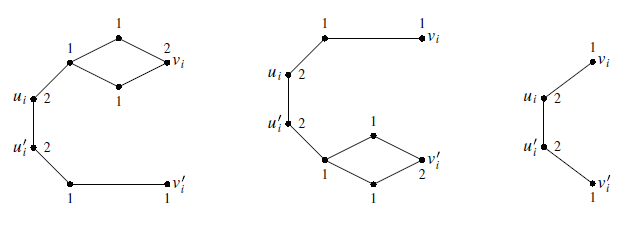
\includegraphics[scale=1]{NPGraph.png}
		\caption{Gadget for each variable $x_{i}$}
		\label{Fig1}
	\end{figure}
\end{center}
We claim that $\phi$ is satisfiable if and only if the optimal target size of $G$ has a size of $n$.

We assume that $\phi$ is satifiable. Define a target set.
\begin{equation}
S = \{{u_{i}| 1\leq i \leq n: x_{i} = true\} \cup \{u_{i}'| 1\leq i \leq n: x_{i} = false}\}
\end{equation}
Note that $|S|=n$. If $u_{i} \in S$, we can see that $v_{i}$ and other nodes between $v_{i}\; and\; u_{i}$ becomes active. The same can be said for $u_{i}'$ and $v_{i}'$. Since we've made the assumption that $\phi$ is satisfiable, by the construction of $G$, all vertices in $W$ become active, which in implies that $v_{i}$ and $v_{i}'$ become active. After this, vertices in $G$ become active.

Let $T$ be the the target set. Suppose that $|T|\leq n$. For any $i = 1,2,...,n$, the threshold of $u_{i}$ and $u_{i}$' is 2. This implies that at least one of them is in $T$. Hence, $|T|=n$ and $T$ does not contain any vertex other than $u_{i},u_{i}'$.

To make $w_{j}$ active, at least of its neighbors have to be active before it. Asumme without loss of generality, $v_{i}$ is active before $w_{j}$. To make $v_{i}$ itself active, we need to have $u_{i}$ active. This implies that $u_{i} \in T$. In summary, if all the vertices in $W$ are active by targeting $T$, the assignment corresponding to $T$ satisfies $\phi$.
Hence, $\phi$ is satisfiable if and only if the optimal target set of $G$ has the size $n$, which would imply that the Target Set Selection problem is NP-hard.\cite{chen}

For the instance of $k=1$ it can be solved trivially. Take any graph $G$ and set of all node's thresholds $k=1$. Activate any of the nodes in that graph and you will create a chain reaction of activating \textbf{every} node in that graph. So, with $k=1$ we can take any one node from that graph that is our target set.\cite{chen}.
\subsubsection{Unanimous Thresholds}
This settings is considered the most influence-resistant of the previously mentioned\cite{chen}. All the nodes have unanimous thresholds  i.e, the threshold of each node is the same as it's degree. This threshold can be applied to an ideal virus-resistant network, where a vertex is infected only if all of its neighbors are infected with the virus. With this in mind, this threshold can be used in constructing robust virus resistant network structures\cite{chen}.
\subsection{Target Set Selection Algorithms compared in this study}

\subsubsection{TIP-DECOMP}
\begin{algorithm}
	\caption{TIP-DECOMP}
	\begin{algorithmic}[1]
		\Require Threshold function, $t$ and social network $G=(V,E)$
		\Ensure $V'$
		
		\ForAll{$vertex \  v_{i}$}
			\State compute $k_{i}$ 
		\EndFor
		\ForAll{$vertex \  v_{i}$}
			\State $dist_{i}=d_{i}^{in}-k_{i} $
		\EndFor
		\State FLAG=TRUE 
		\While{FLAG=TRUE}
			\For{$v_{i} \in V $}
				\If{$v_{i}=min(dist_{i})$}
					\State $v_{i}=$ current $v$
				\EndIf
			\EndFor
			\If{$dist_{j}=\infty$}
				\State FLAG=FALSE 
			\Else
			\State Remove $v_{i}$ from $G$ 
				\ForAll{$v_{j} \in n_{i}^{out}$} 
					\If {$dist_{j}>0$}  
						\State $dist_{j}=dist_{j}-1$
					\Else
						\State$dist_{j}=\infty$  
					\EndIf
				\EndFor
			\EndIf
		\EndWhile
		\State \Return All nodes left in G 
	\end{algorithmic}
\end{algorithm}

\begin{itemize}
	\item $d_{i}^{in}$= degree of vertex $v_{i}$
	\item At lines 1-3, a for loop is used for computing the $k_{i}'s$ for each vertex $v_{i}$. $k_{i}$ is defined as  $k_{i}=[t(v_{i})\cdot d_{i}^{in}]$
	\item At lines 4-6, a for loop is used to compute for the distribution or $dist_{i}$. This will later be used as distinguishing what the current $v_{i}$ is to be used in the inner while loop.
	\item At line 7 a FLAG is instantiated as a boolean variable which will be used in the while loop for identifying the target set selection. We can see it being used in line 8.
	\item The for loop in line 9-13 is for selecting the vertex $v_{i}$ where the result of the degree and the threshold is minimal.
	\item Lines 14-16 are for escaping the main while loop. If this condition is met, it means that the procedure is done.
	\item The else statement in 16-25 is for removing the vertex where the degree and the threshold is almost the same(line 17).
	\item The inner for loop in lines 18-24 is used for updating the distributions in the neighborhood of $v_{j}$.
	\item The process returns the reduced vertex set with the vertices removed if necessary. This is the target set.
\end{itemize}
TIP-DECOMP or Tipping Decomposition is model based on the idea of node "tipping" when a node adopts a property or behavior if a number of his neighbors currently exhibit the same. It is a type of Target Set Selection Algorithm. 

The algorithm above inputs a threshold function $t$ and the social network $G$ and outputs the network with vertices removed based off the condition in the algorithm.\cite{tipdecomp}.
\subsection{VirAds} 


\begin{algorithm}
	\caption{VirAds Algorithm}
	\begin{algorithmic}[1]
		
		
		\Require Graph $G = (V,E),0<\rho<1,d\in N^{+}$
		\Ensure A small $d-seeding$ 
		\State $n_{v}^{(e)} = d(v),n_{v}^{a} = \rho \cdot d(v), r_{v}  = d + 1, v \in V $
		
		\State $r_{v}^{i}=0, i=0..d, P  = \emptyset $
		
		
		\While{there exist inactive vertices}
		\Repeat
		\State $u  = argmax_{v\not\in P}\{n_{v}^{(e)}+n_{v}^{(a)}\}$ 
		
		Recompute $n_{v}^{(e)}$ as the number of new active edges after adding $u$.
		\Until{$u = argmax_{v\not\in P}\{n_{v}^{(e)}+n_{v}^{a}\}$ }
		\State $P  = P \cup \{u\} $
		\State Initialize a queue: $Q  = \{(u,r_{v})\} $
		\ForAll{$x \in N(u)$}
		
		\State $n_{x}^{(a)}  = max\{n_{x}^{a}-1,0\} $
		
		\EndFor
		\While{$Q\not=\emptyset$}
		\State$(t,r_{t})  = Q.pop() $
		\ForAll{$w \in N(t)$}
		\ForAll{$i=r_{t}\  to$ min $\{r_{t}-1,r_{w}-2\}$}
		\State $r_{w}^{i}=r_{w}^{i}+1 $
		\If{$(r_{w}^{(i)}\geq \rho \cdot d_{w})\wedge(r_{w}\geq d)\wedge(i+1<d)$}
		\ForAll{$x\in N(w)$}
		\State $n_{x}^{(a)} =$max$\{n_{x}^{(a)}-1,0\} $	
		\EndFor
		\State $r_{w}=i+1 $
		\If{$w\not\in Q$}
		\State $Q.push(w,r_{w}) $	
		\EndIf
		\EndIf
		\EndFor
		\EndFor
		\EndWhile
		\EndWhile
	\end{algorithmic}
\end{algorithm}
\begin{itemize}
	\item $\rho =$ The influence factor is a decimal between 0-1 that is multiplied to the degree of current vertex $v$ to get $n_{v}^{(a)}$
	\item $r_{v}$ = the round in which the vertex $v$ is activated
	\item $n_{v}^{(e)}=$ the number of new active edges after adding $v$ into the seeding
	\item $n_{v}^{(a)}=$ the number of extra active neighbors $v$ needs in order for it to activate.
	\item $r_{v}^{i}=$ the number of activated neighbors of $v$ up to round $i$ where $i$=$1..d$
	\item Lines 1-2 are for initialization. Line 1 is initialization of variables with values while line 2 is initialization of zero variables.
	\item Line 3 shows that all inactive vertices will be activated or considered in the algorithm
	\item Line 4-6 finds the value where the maximum occurs in the sum of the degree of v and it's effectiveness.
	\item $u$ is added to P in line 7
	\item A queue is initialized by adding the vertex and its corresponding round, which at the start is zero $(u,r_{v})$
	\item Lines 9-11 updates the neighbors of $u$, reducing their degree by 1. If less than zero is reached, it goes back to zero.
	\item At the start of the while loop in line 13 $(t,r_{t})$ is set as the head of the queue. This is obtained by the pop function. 
	\item For all neighbors $w$ of the current node $t$, another for loop is used for checking if the neighbors of $t$ have reached the threshold defined by $\rho \cdot d_{w}$ AND $round \; r_{w} \geq the\; max\; round\; d$ AND the index $i$ of the for loop doesn't exceed the max rounds $d$.
	\item This then leads to the thresholds of the neighbors of the that neighbor $w$ being decremented.
	\item In line 21 the round of the neighbor $w$ is incremented and if that current $w \notin Q$ then it is added to the queue and the while loop starts again.
\end{itemize}
VirAds selects in each step the vertex $u$ with the highest effectiveness which is defined as $n^{(e)}_{u}+n^{(e)}_{a}$. Which is basically the vertex $v$ which can activate the most number of $edges$. It also considers the vertex with the most active neighbors. After that, the algorithm updates the measures for all the remaining vertices. VirAds will make the selection based on the information within $d$-hop neighbor around the considered vertices rather than only one-hop neighbor as in the degree-based heuristic. When a vertex $u$ is selected, it causes a chain-reaction and activate a sequence of vertices or lower the rounds in which vertices are activated\cite{virads}.

The algorithm utilizes a queue. A queue is a data structure which is FIFO. Imagine, a line at any commercial establishment where the first who came is the first who's served. 
\newpage